\documentclass[output=paper,draft,draftmode,colorlinks,citecolor=brown]{langscibook}
\ChapterDOI{10.5281/zenodo.7353603}

\author{Marielle Butters\affiliation{University of Colorado at Boulder}}
\title{The negative existential cycle in Chadic}


\abstract{Chadic languages, like languages of West and Central Africa more generally, are known to make use of typologically rare negation strategies. Not only do many Chadic languages exhibit bi-partite negation, there is also a tendency for the second of these two verbal negators to occur after the verb, in contrast to a cross-linguistic preference for pre-verbal negation. This particular study examines the extent to which Croft's \citeyearpar{Croft1991} Negative Existential Cycle (NEC) may be demonstrated across Chadic languages. Furthermore, the study explores the use of the NEC as an explanatory framework in determining sources and pathways of verbal negation in Chadic languages. An important implication of this study is that identification of the B{\textasciitilde}C stage of the NEC elucidates the relationship between verbal negation and negative existential predication, as well as the relationship between these domains and other domains of the grammar such as aspect.

\keywords{Chadic, negation, existential predication, cyclical change}
} 


\IfFileExists{../localcommands.tex}{
   % add all extra packages you need to load to this file

\usepackage{tabularx,multicol}
\usepackage{url}
\urlstyle{same}

\usepackage{listings}
\lstset{basicstyle=\ttfamily,tabsize=2,breaklines=true}

\usepackage{langsci-optional}
\usepackage{langsci-lgr}
\usepackage{langsci-gb4e}

%from elena-----------------------------------
\usepackage{pgfplots,pgfplotstable}
\definecolor{lsDOIGray}{cmyk}{0,0,0,0.45}
\usepackage{xassoccnt}
\newcounter{realpage}
\DeclareAssociatedCounters{page}{realpage}
\AtBeginDocument{%
  \stepcounter{realpage}
}
\usepackage{enumitem}
\usepackage[]{longtable}
\usepackage{comment}

%from Nina K.---------------------------------
\usepackage{csquotes}
%\usepackage{expex}
\pgfplotsset{compat=1.16} % Why?
% \usepackage{xeCJK}
% \setCJKmainfont{HanaMinA}
\usepackage{rotating}
\usepackage{colortbl}
\usepackage{multirow}
\usepackage{dirtree}

%from Niina-----------------------------------
\usepackage{verbatim}
\usetikzlibrary{intersections, backgrounds, shapes, angles, quotes,
decorations.pathmorphing, arrows.meta, decorations.text, tikzmark}
% positioning and calc are loaded by document class
	\tikzset{snake it/.style={decorate, decoration=snake}}
\usepackage{tikz-qtree}

% figures side-by-side with body text:
\usepackage{wrapfig}
\usepackage{subcaption}

%\usepackage{enumerate}
%\usepackage[nonumberlist]{glossaries}


\usepackage[linguistics,edges]{forest}
\usetikzlibrary{positioning}
\usepackage{soul}
\usepackage{langsci-bidi}
\usepackage{langsci-branding}

   \newcommand*{\orcid}{}

%-------------------from Elena------------------------------------------------------------

\newcommand{\appref}[1]{Appendix \ref{#1}}
\newcommand{\fnref}[1]{Footnote \ref{#1}} 

\newenvironment{langscibars}{\begin{axis}[ybar,xtick=data, xticklabels from table={\mydata}{pos}, 
        width  = \textwidth,
	height = .3\textheight,
    	nodes near coords, 
	xtick=data,
	x tick label style={},  
	ymin=0,
	cycle list name=langscicolors
        ]}{\end{axis}}
        
\newcommand{\langscibar}[1]{\addplot+ table [x=i, y=#1] {\mydata};\addlegendentry{#1};}

\newcommand{\langscidata}[1]{\pgfplotstableread{#1}\mydata;}


% for annotations above example lines:
\newcommand{\overnote}[1]{\makebox[0pt][l]{\raisebox{\baselineskip}{\upshape
#1}}}
\newcommand{\moreovernote}[1]{\makebox[0pt][l]{\raisebox{2\baselineskip}{\upshape #1}}}

%--------------------from Niina----------------------------------------------------------

% \makeatletter
% \def\blx@maxline{77}
% \makeatother

% An Arabic font added to `fonts' folder, it's free and open-source
% When run on Windows, LaTeX may need the complete file name of the font:
% Amiri-Regular.ttf
% \newfontfamily\arabfont{Amiri}
% \newcommand\textarab[1]{{\arabfont #1}}%%% \textarab{...}




\newcommand{\todoref}[1]{\todo[color=green!40]{#1}}%%% 
\newcommand{\todofix}[1]{\todo[color=blue!40]{#1}}%%% 

\DeclareBibliographyCategory{sources}% filter some references
\DeclareBibliographyCategory{online}

% draw a thick bar of desired length (used for visual presentation in a
% tabular)
\newcommand{\cocabar}[1]{\color{gray}\rule[1pt]{{#1}mm}{1ex}}

% to preserve original formatting in an appendix:
\newenvironment{unindented}[0]{\setlength{\parindent}{0pt}\setlength{\parskip}{1ex
plus 0.5ex minus 0.2ex}}{}
% for annotations above example lines:
%\newcommand{\overnote}[1]{\makebox[0pt][l]{\raisebox{\baselineskip}{\upshape
%#1}}}
%\newcommand{\moreovernote}[1]{\makebox[0pt][l]{\raisebox{2\baselineskip}{\upshape #1}}}

\definecolor{blech}{rgb}{.78,.78.,.62}
\definecolor{ochre}{cmyk}{0, .42, .83, .20}
\newcommand{\exem}[1]{\textit{\textbf{#1}}}
\newcommand{\glem}[1]{\MakeUppercase{\scriptsize{\textbf{#1}}}} 
\newcommand{\denote}[1]{\mbox{$[\![\mbox{#1}]\!]$}}

\newcommand{\stacktwo}[2]{\makebox[0pt][l]{\hspace{.5pt}#1}#2}

%------------------from Nina K.-------------------------------

\newcommand{\citealtv}[1]{\citealt{#1} [this volume]}


% \renewcommand{\textdblhyphen}{⹀}


% \newcommand{\ꜥ}{\textsf{ꜥ}}
\newcommand{\ꜥ}{ʿ}
\newcommand{\ꜣ}{\kern-.25pt\texttt{ꜣ}\kern-.6pt}


\makeatletter
\let\thetitle\@title
\let\theauthor\@author
\makeatother


\newcommand{\togglepaper}[1][0]{
   \bibliography{../localbibliography}
   \papernote{\scriptsize\normalfont
     \theauthor.
     \titleTemp.
     To appear in:
     Change Volume Editor \& in localcommands.tex
     Change volume title in localcommands.tex
     Berlin: Language Science Press. [preliminary page numbering]
   }
   \pagenumbering{roman}
   \setcounter{chapter}{#1}
   \addtocounter{chapter}{-1}
}


\newfontfamily\arabicfont[Script=Arabic,ItalicFont=*,Scale=1.4]{ScheherazadeRegOT_Jazm.ttf}
% \newcommand{\arabscript}[1]{\RL{\Parsifont #1}}
\newcommand{\textarab}[1]{{\arabicfont #1}}



\DeclareCiteCommand{\textCitetv}
  {\usebibmacro{prenote}}
  {\ifciteindex
     {\indexnames{labelname}}
     {}%
   \printtext[bibhyperref]{\printnames{labelname}\addspace\bibopenparen\printfield{year}}}
  {\multicitedelim}
  {\printtext[bibhyperref]{\usebibmacro{postnote}\addspace[this volume]\bibcloseparen}}


\colorlet{karlgrencol}{pink}
\colorlet{normancol}{green}
\colorlet{pancol}{blue}
\colorlet{ohtacol}{gray}
\colorlet{peyraubecol}{orange}
\colorlet{peyraubecolmod}{yellow}
\colorlet{wangcol}{red}

\DeclareNewSectionCommand
  [
    counterwithin = appendixsubsection,
    beforeskip=-10pt,
    afterskip=1sp,
    indent = 0pt,
    font = \usekomafont{subsubsection},
    level = 3,
    tocindent = 7.0em,
    toclevel = 3,
    tocnumwidth = 4.1em,
    tocstyle = section,
    style = section
  ]
  {appendixsubsubsection}

   %% hyphenation points for line breaks
%% Normally, automatic hyphenation in LaTeX is very good
%% If a word is mis-hyphenated, add it to this file
%%
%% add information to TeX file before \begin{document} with:
%% %% hyphenation points for line breaks
%% Normally, automatic hyphenation in LaTeX is very good
%% If a word is mis-hyphenated, add it to this file
%%
%% add information to TeX file before \begin{document} with:
%% %% hyphenation points for line breaks
%% Normally, automatic hyphenation in LaTeX is very good
%% If a word is mis-hyphenated, add it to this file
%%
%% add information to TeX file before \begin{document} with:
%% \include{localhyphenation}
\hyphenation{
    Af-ri-caans
    Bar-tens
    cen-tu-ry
    comitative-existential
    com-ple-ments
    data-set
    dia-chro-nic
    ex-is-ten-tial
    ex-is-ten-tials
    Fraj-zyn-gier
    Has-pel-math
    Hol-ton
    Jes-per-sen
    lo-ca-ti-ve-ex-is-ten-tial
    Ma-khu-wa
    mar-ker
    Nai-khin
    negat-ed
    part-ti-ci-ple
    Swa-hi-li
    Ve-se-li-no-va
}

\hyphenation{
    Af-ri-caans
    Bar-tens
    cen-tu-ry
    comitative-existential
    com-ple-ments
    data-set
    dia-chro-nic
    ex-is-ten-tial
    ex-is-ten-tials
    Fraj-zyn-gier
    Has-pel-math
    Hol-ton
    Jes-per-sen
    lo-ca-ti-ve-ex-is-ten-tial
    Ma-khu-wa
    mar-ker
    Nai-khin
    negat-ed
    part-ti-ci-ple
    Swa-hi-li
    Ve-se-li-no-va
}

\hyphenation{
    Af-ri-caans
    Bar-tens
    cen-tu-ry
    comitative-existential
    com-ple-ments
    data-set
    dia-chro-nic
    ex-is-ten-tial
    ex-is-ten-tials
    Fraj-zyn-gier
    Has-pel-math
    Hol-ton
    Jes-per-sen
    lo-ca-ti-ve-ex-is-ten-tial
    Ma-khu-wa
    mar-ker
    Nai-khin
    negat-ed
    part-ti-ci-ple
    Swa-hi-li
    Ve-se-li-no-va
}

   \togglepaper[1]%%chapternumber
}{}


\AffiliationsWithoutIndexing{}

\begin{document}
\maketitle

\section{Introduction}\label{sec:3:1}

In this paper, I consider the applicability of the types and stages of \citegen{Croft1991} Negative Existential Cycle (henceforth NEC) to the Chadic\il{Chadic|(} language family -- a family which already exhibits a cross-linguistically unusual negation system. In Croft's framework, there are three types of languages, A, B, and C that form a diachronic cycle. The direction of change is A{\textasciitilde}B, B{\textasciitilde}C, and C{\textasciitilde}A, where a special negative existential form arises, subsequently comes to be used as a verbal negator, and is then supplemented by a positive existential so that it is restored to a regular negative + existential construction. In brief, these internally variable stages represent historical changes in process as negative existential predication comes to mark verbal negation. Croft's types and stages are summarized here:

% % \begin{quote}
\begin{description}
\item[Type A:] There is no special negative existential predicate. The affirmative existential predicate is negated by the ordinary verbal negator.
\item[A{\textasciitilde}B:] A special negative existential predicate is found in addition to the regular negative existential form. 
\item[Type B:] There is a special negative existential marker that is distinct from the ordinary verbal negator. 
\item[B{\textasciitilde}C:] The negative existential predicate begins to be used for ordinary verbal negation, but is restricted to specific contexts. 
\item[Type C:] The negative existential predicate is identical in form and position to the verbal negator.
\item[C{\textasciitilde}A:] The negative-existential-cum-verbal-negator is in the process of being reanalyzed as only a negative marker and a regular positive existential verb begins to be used with it in negative existential constructions.
\end{description}
% % \end{quote}

I find examples of most -- though not all -- of these types and stages in the Chadic family. However, while some languages fit neatly into given stages, this work follows previous scholarship (e.g. \citealt{Veselinova2016}) in suggesting that languages sometimes exhibit overlap between types or stages.  Beyond identification of the NEC in Chadic, a goal of this paper is to suggest that an exploration of the NEC is illuminative in identifying sources of verbal negation, taking the Chadic family as an example. In Chadic, there is great variation in the expression of negation in terms of phonological and morphological form as well as the number of markers used in negative constructions. Existential predication appears to be one pathway through which new forms come to serve as verbal negators. 

All data included in this paper comes from available grammars. According to
Glottolog \citep{HammarstromBank2018}, there are roughly 200 Chadic
languages. These are spoken across northern Nigeria, southern Niger,
Southern Chad, the Central African Republic, and parts of Northern
Cameroon. Of these, there exist an approximate 60 available grammars or
grammatical sketches. Following \citet{Newman2000}, these languages can be
divided into four subgroups: Western, Central, Eastern, and Masa. There is
an unequal distribution of languages across the family with the largest
numbers belonging to the Western and Central subfamilies and a mere ten
languages belonging to Masa. Scholarship has largely favored Western and
Central languages and these comprise the majority of languages presented in
this paper. The languages included herein were selected primarily through
convenience. Upon perusal of the approximate 30 grammars available to me, I
was able to determine evidence of the cycle in 12 of these languages, three
from the Western branch, eight from the Central branch, one from the Eastern branch, and none from
Masa. Some grammars were produced several decades ago, meaning the level
of description and inclusion of evidence fall below contemporary standards;
namely, some grammars included unglossed examples with little to no
accompanying contextual information. In cases where there are no glosses, I
have reconstructed them myself.  

The organization of the paper is as follows. I begin with a brief
introduction of interesting issues within the Chadic negation system. This
is followed by a presentation of examples of languages within each of the
types and stages of the NEC. I then submit some examples of languages that
do not fit neatly into any one type or stage. This is followed by a
discussion of the implications of the data as a whole. In the final
section, I propose common sources for verbal negators in Chadic and discuss
the merits of including existential predication as one of these sources.

\section{Negation in Chadic languages}\label{sec:3:2}

Before addressing the NEC, it should be acknowledged that the verbal
negation system itself is quite unusual in Chadic. In a study on the
distribution of negative word order, \citet{Dryer2009} finds that VO \&
V\textsubscript{NEG} languages -- those where the negative marker follows
the verb -- are a typological phenomenon unique to Central Africa
(Niger-Congo, Nilo-Saharan, and Chadic) and, to a
lesser extent, to New Guinea. Though there are isolated cases of VO \&
V\textsubscript{NEG} languages around the world, there is nowhere with such
a concentration of examples as is found in these two regions. It has been
observed as early as \citet{Jespersen1917} that there is a cross-linguistic
preference for negators to occur directly before the verb, yet in Chadic
languages, which are most frequently but not always SVO, the negative marker occurs not only
after the verb, but in the final position of the clause. In the great
majority of cases, the verb may be followed only by time adverbials and
interrogatives. 

Additionally, many languages across the Chadic family employ bi-partite negation
markers, though Proto-Chadic negation appears to have been single-mar\-ked in clau\-se-fi\-nal
position \citep{Newman1977}. In his classic study of negation,
\citet[92]{Dahl1979} finds that where there is bi-par\-ti\-te negation in his sample,
the two negators nearly always surround the verb. He takes this to suggest
a general tendency for negators to occur as close to the finite element of
the clause as possible. Yet this is rarely what happens
 for Chadic, as the
first negator in these languages often occurs before the subject and the second
negator often occurs after the object where the dominant word order is SVO.
Indeed, \citet[95]{Dahl1979} cites West African languages as typologically
unusual among his sample.

%There is still much to be discovered regarding negation in Chadic, including the sources and pathways behind the various forms that occur.

\section{The negative existential cycle across Chadic languages}\label{sec:3:3}

In Chadic languages, given the sparsity of resources and examples provided
in many grammars of individual languages, it is difficult to get a sense of
language change over a long period of time. Thus, rather than focusing on
the evolution of negation within individual languages, the focus of this
study is on evidence of the stages of NEC across the Chadic language
family. 

The NEC, as an explanatory framework, illuminates the relationship between
the domain of negative existentials and of verbal negation. Negative
existential predicators differ from verbal negators by virtue of the fact
that they indicate a state rather than an action or a process; they serve
to express the absence of an entity and to pragmatically remove a referent
from the scene \citep{Veselinova2013}. Verbal negation, on the other hand,
refers to the negation of a declarative clause with a verbal predicate in the
sense of \citet{Dahl2010} and \citet{Miestamo2005}. Given the differing
functions, these domains are constantly formally distinguished, though they also interact
closely. In this section, I present examples of Chadic languages that
fit each of the types and stages of the NEC.

\subsection{Type A}\label{sec:3:3.1}

In Type A languages there is no special negative existential predicator,
but the negation of the affirmative existential is performed by the verbal
negator. This type appears to be particularly widespread in Chadic languages, appearing in at least a dozen languages surveyed, though not all are represented in this chapter for the sake of space. In \ili{Pa'anci}, a West
Chadic language, the affirmative existential \textit{ani} occurs with the
regular verbal negator \textit{wa} to negate existence, as in
\REF{ex:paanci-water}.  The negator \textit{wa} also occurs in final
position in utterances with verbs and is followed only by a
sentence-level emphatic particle \textit{na}, as in \REF{ex:paanci-come}.
\citet[102]{Skinner1979} notes that \textit{ani} is derived from a
``locative verb feature bundle'' \textit{ánà,} followed by an
associative preposition \textit{i}. \REF{ex:paanci-corn} is an example of
an affirmative existential utterance.  

\newpage
\ea\label{ex:paanci-water-come-corn}
\langinfo{Pa'anci}{}{\citealt[102, 150]{Skinner1979}}

\ea\label{ex:paanci-water}

\gll \textbf{ani} ambi \textbf{wa}\\
one.\textsc{cont.assoc} water \textsc{neg}\\

\glt `There is no water.'{\footnotemark}
\footnotetext{All Pa'anci glosses were constructed by the author.} 
\ex\label{ex:paanci-come} 

\gll ná munde na dava \textbf{wa} na\\
3\textsc{sg} say 3\textsc{sg} come \textsc{neg} \textsc{emph}\\ 

\glt `He said he did not come.'
\ex\label{ex:paanci-corn}

\gll \textbf{ani} aci aɦari pangwa\\
one.\textsc{cont.assoc} guinea.corn inside corn.bin\\ 

\glt `There is guinea corn in the bin.'
\z
\z

It should be noted that \textit{ani} and \textit{wa} occur at opposite ends of the clause. The distance of the verbal negator from the existential predicate suggests the separate functional domains of negation and existential predication, making the frequency of Type A understandable.

In \ili{Gidar}, a Central Chadic language, the affirmative existential verb \textit{t\`ɑ} (derived from the copula) must co-occur with the verbal negator \textit{ɓà} in order to mark negative existence, as in \REF{ex:gidar-want}. The marker \textit{tà} is purely existential and does not code existence in a location. All negative clauses in Gidar are marked by the clause-final particle \textit{ɓà}, as in \REF{ex:gidar-chief}. \REF{ex:gidar-desire} is an example of an affirmative existential utterance.

\ea\label{ex:gidar-want-chief-desire}
\langinfo{Gidar}{}{\citealt[251, 311, 309]{Frajzyngier2008}}

\ea\label{ex:gidar-want}

\gll ɗ\'əf \textbf{tà}-y án d\`ə-dàw kàyí-t \textbf{ɓà}\\
man be-3\textsc{m} \textsc{rel} 3\textsc{m}-\textsc{dep.prog} want-3\textsc{f} \textsc{neg}\\

\glt `There is no man who wants her.'
\ex\label{ex:gidar-chief}

\gll {mə̩̀lìy} d\`ə-dàw dáw sá \textbf{ɓà}\\
chief 3\textsc{m}-\textsc{dep.prog} walk even \textsc{neg}\\

\glt `The chief didn't even walk.'
\ex\label{ex:gidar-desire}

\gll ɗíi \textbf{tà}-ŋ d\'ə-dà{\op}w{\cp} káí-t\'ə-nì\\
men be-3\textsc{pl} 3\textsc{m}-\textsc{dep.prog} want-3\textsc{f}-\textsc{pl}\\

\glt `There are many men who desire her.'

\z
\z

As there is no special negative existential form in \ili{Gidar}, it is clearly a Type A language. 

\subsection{A{\textasciitilde}B}\label{sec:3:3.2}

In this synchronically variable stage, there is a special negative existential form in addition to the regular negative existential form. \citet[7]{Croft1991} describes the special negative existential as ``usually but not always a contraction or fusion of the verbal negator and the positive existential form''.

In \ili{Hausa}, a West Chadic language, there are two negative existential
forms, \textit{bâ} and \textit{b\=abù}, shown in \REF{ex:hausa-remain},
which are distinct in quantity and tone from the bi-partite verbal negator
\textit{b\=a\ldots{}ba} used in tenses, aspects, and moods other than continuous
and subjunctive, as in \REF{ex:hausa-pay}.  In negative continuous
utterances, the verbal negator is \textit{b\=a}. Generally, the two
negative existentials may be used interchangeably, though the former occurs
more frequently when there is a nominal predicate. When there is no overt
object, only \textit{b\=abù} can be used. The word \textit{b\=abù} is
also sometimes used colloquially to mean `no', often as an elliptical
response.  The affirmative existentials in
\ili{Hausa}, \textit{à{}kwai} and \textit{dà}, as in \REF{ex:hausa-stranger}
and \REF{ex:hausa-money}, bear no resemblance to the
negative existentials nor to the verbal negators. However, like the
negative existential predicator, both occur in phrase-initial position.%
%
\footnote{\textit{dà} is also the morpheme used for the preposition 'with'.
While \textit{dà} is followed by an independent pronoun, \textit{àkwai} makes use of weak object pronouns. Furthermore, \textit{dà}, unlike \textit{àkwai}, can never be stranded unless it is followed by \textit{àkwai}; indeed, in some dialects, \textit{dàkwai} has fused into a single word, cf. \citet{Newman1971}.}

%
\ea Hausa \citep[178--179, 357]{Newman2000}%#\label{ex:hausa-remain-pay-stranger-money}
\\
\label{ex:hausa-remain-pay-stranger-money}

\ea \label{ex:hausa-remain}

\gll \textbf{bābù/bâ} sauran àbinci\\
  	\textsc{neg.ex} other food\\

\glt ‘There is no food remaining.’\footnote{All Hausa glosses have been constructed by the author.}
  \ex \label{ex:hausa-pay}

\gll \textbf{bà} zā mù biyā sù \textbf{ba}\\
  	\textsc{neg} \textsc{fut} 1\textsc{pl} pay 3\textsc{pl} \textsc{neg}\\

\glt `We will not pay them.'
  \ex \label{ex:hausa-stranger}

\gll \textbf{àkwai} wani bā̀ƙō à kōfā̀ \\
  	\textsc{ex} \textsc{indf} stranger \textsc{prep} door\\
\glt `There is a stranger at the door.'
  \ex \label{ex:hausa-money}

\gll \textbf{dà} kuɗɪ̄\\
  	\textsc{ex} money\\
\glt `There is money.'
\z
\z


In \ili{Hausa}, then, there is a second negative existential form, but there is no evidence that this is the result of fusion with an affirmative existential. \citet{Newman2000} addresses the dispute regarding the relation between \textit{b\=abù} and \textit{bâ}. Some, such as \citet{Eulenberg1971}, take \textit{b\=abù} as the original and \textit{bâ} to be a phonologically reduced form.  \citet{Newman1971}, however, proposes that the source for this alternate form \textit{bābù} is a fusion, \textit{bâ} \textsc{neg} \textit{+} \textit{\=abù} `thing', a change attested in other Chadic languages as well. As evidence against \textit{b\=abù} as basic, he cites the fact that it takes independent rather than object pronouns as its complement. Additionally, Newman notes that \textit{bâ} might have been borrowed from \ili{Kanuri}, as the negative existential therein is of the same shape.

It is possible that \textit{bâ} is losing its distinction as a negative
existential, given its resemblance to the clause-initial verbal negator
\textit{bà,} lending to the fusion of a new form \textit{b\=abù} to be
preferred in certain areas of the grammar as a solution to ambiguity.
Evidence for this lays in the use of \textit{b\=abù} in emphatic
utterances, as in dispute and disagreement. \citet{Croft1991} discusses
the ``close diachronic association'' between negative existentials,
negative interjections and verbal negators in connection with this stage.
\ili{Hausa} is of A{\textasciitilde}B because there is a second negative
existential form which has some restricted uses.

In \ili{Lele}, an East Chadic language, the locative anaphora,
\textit{màní},\footnote{It should be noted that the primary role of
\textit{màní} is locative anaphora, though it is used on occasion to
mark affirmative existence as in the examples given.}, which is also used to mark
affirmative existence, as in (\ref{ex:lele-god}) and (\ref{ex:lele-corn}). This
form can be negated by the verbal negator, \textit{ɗé}, as in
\REF{ex:lele-no-god}, in accordance with Type A. Additionally, there is a
form \textit{wíléŋ} `lack' which serves as a negative existential,
as in \REF{ex:lele-still-no-god}.  

\ea\label{ex:lele-god-corn-no-god}
\langinfo{Lele}{}{\citealt[196]{Frajzyngier2001}}\\ 

\ea\label{ex:lele-god}

\gll kùmnó \textbf{màní}\\
God there\\

\glt `God exists'
\ex\label{ex:lele-corn} 

\gll ɗíglè káŋ kàsà
\textbf{màní}\\ year \textsc{dem} corn there\\

\glt `there is corn this year'
\ex\label{ex:lele-no-god} 

\gll kùmnó \textbf{màní} \textbf{ɗé}\\
God \textsc{ex} \textsc{neg}\\ 

\glt `God does not exist'
\ex\label{ex:lele-still-no-god} 

\gll kùmnó \textbf{wíléŋ}\\
God \textsc{neg.ex}\\ 

\glt `God does not exist'
\z
\z

Given that the form \textit{màní…ɗé} can be substituted for \textit{wíléŋ} in the same utterance, there does not appear to be restriction of these forms.

\subsection{Type B}\label{sec:3:3.3}

In Type B there is a special negative existential marker which is distinct
from the verbal negator. \ili{Muyang}, a Central Chadic language, is
exemplary of this type. Here, the negative existential \textit{b\=\i}
differs from the affirmative existential, as in \REF{ex:muyang-none}, and
the existential \textit{bù}, as in \REF{ex:muyang-some} differs from the verbal
negator \textit{d\`o}, as in \REF{ex:muyang-cry}.  

\ea\label{ex:muyang-none-some-cry}
\langinfo{Muyang}{}{\citealt[27, 118]{SmithGravina2010}}

\ea\label{ex:muyang-none}
\gll \=a-\textbf{b\=\i}\\
3\textsc{sg}-\textsc{neg.ex}\\
\glt `He/she is not there.' or `There isn't
any.' \ex\label{ex:muyang-some}
\gll \=a-\textbf{bù}\\
3\textsc{sg}-\textsc{ex}\\
\glt `He/she is there.' or `There is some.'
\ex\label{ex:muyang-cry}
\gll k\=a-ɮ\=ax \textbf{d\`o}\\ 2\textsc{sg}-roar
\textsc{neg}\\
\glt `You do not cry out.'
\z
\z

A perhaps less obvious example of a language belonging to Type B is
\ili{Mina}, a Central Chadic language where the negative existential
construction appears to be diachronically young. Verbal negation in Mina is
marked by a clause final particle \textit{skù}, as in \REF{ex:mina-good}.
The verbal negator has scope over the entity immediately preceding it. The
affirmative existential \textit{ɗáhà} (often shortened to
\textit{ɗá}) must co-occur with the verbal negator \textit{skù} to
create a negative existential predicate, as in \REF{ex:mina-wet}. Mina
differs from other Chadic languages in that the existential predicate and
the verbal negator neighbor one another. It may be that this fact
contributes to the clipped \textit{ɗà} existential form in negative existential
predicates that is typically in its full form in affirmative existentials
as in \REF{ex:mina-granary}.  

\ea\label{ex:mina-good-wet-granary}
\langinfo{Mina}{}{\citealt[46, 66, 261, 267]{FrajzyngierJohnston2005}}\\ 

\ea\label{ex:mina-good}

\gll á t{ì}-y-á-h hà nék \textbf{skù}\\
3\textsc{sg} see-\textsc{go}-2\textsc{sg} 2\textsc{sg} good \textsc{neg}\\ 

\glt `He does not see you as a good person.'
\ex\label{ex:mina-wet} 

\gll kó m\`ə l\'əɓ-{yíì} \textbf{ɗá} \textbf{skù}\\
\textsc{quant} \textsc{rel} wet-\textsc{pl} \textsc{ex} \textsc{neg}\\ 

\glt `Not even one [page] was wet.'
\ex\label{ex:mina-granary}

\gll tèbéŋ t\'ə nd{ì}r \textbf{ɗáhà}\\
granary \textsc{gen} sorghum \textsc{ex}\\

\glt `There is a granary of sorghum.'
\ex\label{ex:mina-superior}

\gll m\'ə mb\'əɗ z\'ə v-{yíì} \textbf{ɗà} skù\\
\textsc{rel} surpass \textsc{ee} who-\textsc{pl} \textsc{ex} \textsc{neg}\\

\glt `Who is superior? Nobody.'

\z
\z

It appears from the available data that \textit{ɗá} \textit{skù} is
coming to serve as its own lexical unit. Evidence for this is provided by
\REF{ex:mina-superior} where \textit{ɗá skù} can constitute a complete
clause. \citet{Haspelmath1997} finds that it is not uncommon for negative
existentials to perform the function of indefinite pronouns in many Oceanic
languages.

Though the negative existential form here is transparent, it appears to be
stable. 

\subsection{B{\textasciitilde}C}\label{sec:3:3.4}
\citet[9]{Croft1991} calls this synchronic variable stage ``the most important step in support of our hypothesis'', and it certainly seems to generate the most interesting questions. Here, the negative existential predicator begins to be used for ordinary verbal negation. The negative existential may compete with the verbal negator, sometimes being used instead of it. 

\ili{Hdi}, a Central Chadic language, is probably the best example of this
stage. Here, verbal negation is typically marked by \textit{á} \ldots{}
\textit{wà/wù} as in \REF{ex:hdi-school}. The forms \textit{wà} and
\textit{wù}, are free variants, though some speakers show preference for
one or the other. The affirmative existential is \textit{màm\'u}
(sometimes reduced to \textit{màá}) and cannot occur with the verbal
negator, as in \REF{ex:hdi-marriage}.  In order to negate existence, the
form \textit{xàɗ\'u} `lack' is used with a single negative marker at the
end of the clause, as in \REF{ex:hdi-rain}.
  
Additionally, there is evidence that \textit{xàɗ\'u} is coming to replace
the first verbal negator, not just in existential utterances, but in verbal
utterances as well. \citet{FrajzyngierShay2002} note that \textit{xàɗ} codes negative subjunctive in
imperfective as well as negative imperfective in the indicative mood, as in
\REF{ex:hdi-look}.  These authors also state that the \textit{xàɗ
\ldots{} wà} frame codes ``pragmatically dependent negative clauses'',
such as negative relative clauses, negative conditional protases, and
negative conditional and temporal apodoses as well as concluding clauses after another statement has been made, as in
\REF{ex:hdi-catch}.

\newpage
\ea\label{ex:hdi-school-marriage-rain-look-catch}
\langinfo{Hdi}{}{\citealt[41, 89, 152, 380, 385]{FrajzyngierShay2002}}\\

\ea\label{ex:hdi-school}
\gll ɗvà \textbf{`á} xdí-xà tá
l'école \textbf{wù}, ká-'á\\ like \textsc{neg} Hdi-\textsc{pl}
\textsc{obj} {school (Fr.)} \textsc{neg} \textsc{comp-3sg}\\
\glt `{}``Hdi do not like school,'' he said.'
\ex\label{ex:hdi-marriage}
\gll índà
dimanche ná \textbf{màm\'u} marriage ndánà\\ every {Sunday (Fr.)}
\textsc{comp} \textsc{ex} marriage now\\
\glt `Every Sunday there is a marriage now.'
\ex\label{ex:hdi-rain}
\gll \textbf{xàɗ\'u} {ì}mí{}
\textbf{wà}\\ lack water \textsc{neg}\\
\glt `There are no rains.'
\ex\label{ex:hdi-look}
\gll \textbf{xàɗ}-ká kà \`nghá tsá
\textbf{wà}\\ lack-2\textsc{sg} \textsc{seq} look \textsc{def}
\textsc{neg}\\
\glt `You should not look at it.' \ex\label{ex:hdi-catch}

\gll \textbf{xàɗ} x\`əŋ tà ksá-f-tà dágálá \textbf{wà}\\
lack 3\textsc{pl} \textsc{ipfv} catch-up-\textsc{ref} many \textsc{neg}\\

\glt `They do not catch many.'
\z
\z There may be something similar
beginning to happen in \ili{Wandala}, though this is underdeveloped.
\ili{Wandala} is a Central Chadic language where verbal negation is marked
by \textit{k} (clause-internally) or \textit{kà} (when in clause-final
position). The negator is placed after the verb and before the nominal
subject or object, as in \REF{ex:wandala-stop}, which exhibits VSO word order. Only when the verb is not
followed by an argument does the negative particle occur clause-finally.
Negative existential clauses are formed through the use of
\textit{ɓákà} or \textit{ɓáakà} in clause-initial or clause-final
position, depending on whether the information presented is old or new, as
in \REF{ex:wandala-words}. 
  
Generally, the negative existential and the verbal negator do not co-occur, though there are some rare instances in which they do, as in \REF{ex:wandala-means}. It is unclear what function is served by combining these elements, but it is possible that the final \textit{kà} here is simply a clipped form of the negative existential, as there are cases where the negative existential is repeated, as in \REF{ex:wandala-surpass}.

\ea\label{ex:wandala-stop-words-means-surpass}
\langinfo{Wandala}{}{\citealt[85, 208, 436, 583]{Frajzyngier2012}}\\ 

\ea\label{ex:wandala-stop}

\gll tsà-n-á \textbf{k} nábbà\\
stop-3\textsc{sg-go} \textsc{neg} Nabba\\ 

\glt `He did not stop Nabba.'
\ex\label{ex:wandala-words}

\gll á yà-wá \'əlvà-á-rwà \textbf{ɓákà}\\
well 1\textsc{sg-com} word-\textsc{gen-1sg} \textsc{neg.ex}\\

\glt `Well, I have no words.'
\ex\label{ex:wandala-means}

\gll ŋán kín{ì} sé à hàyà bà dó n\`ə ŋánnà \textbf{ɓákà} péɗà-á-r nà \textbf{kà}\\
3\textsc{sg} \textsc{cntr.foc} only 3\textsc{sg} like \textsc{foc} man \textsc{dem} \textsc{def} \textsc{neg.ex} means-\textsc{gen-3sg} \textsc{dem} \textsc{neg}\\

\glt `She, she likes only the man that does not have any means.' [or `only useless men']
\ex\label{ex:wandala-surpass}

\gll \textbf{ɓákà} ùrà tà tàttàyà à j-\'u g-íyà \textbf{ɓákà}\\
\textsc{neg.ex} person 3\textsc{pl} search 3\textsc{sg} surpass-\textsc{vent} to-\textsc{1sg} \textsc{neg.ex}\\

\glt `One does not look for a person to surpass me.'

\z
\z

The open question that emerges from the data from \ili{Hdi} (and, to a lesser extent, from \ili{Wandala}) is what purpose is served by the enforcement of the verbal negator by the negative existential.

\subsection{Type C}\label{sec:3:3.5}

In Type C, the negative existential is identical in form and position to the verbal negator, demonstrating ``polysemy between negative existential meaning and verbal negation'' \citep[12]{Croft1991}. This occurs rarely in Chadic languages, but appears in \ili{Gude}, a Central Chadic language. 

In all TAM in \ili{Gude}, the verbal negator, \textit{pooshi,} exactly
resembles the negative existential, \textit{pooshi}, as exhibited by the
negated verbal phrase in \REF{ex:gude-stone} and the negative existential
utterance in \REF{ex:gude-chief}.  The negative existential does not appear
related to the affirmative existential \textit{tə'i}; rather,
\citet[90]{Hoskison1983} suggests that \textit{pooshi} is formed from
\textit{pə} used in phrases of refusal and \textit{uushi} `thing', as also
attested in \ili{Hausa} above. In the completive aspect, there is an
alternative verbal negation strategy which uses \textit{ma{\ldots}mə}
surrounding the verb stem, as in \REF{ex:gude-Musa}, which follows VSO word order unlike the other examples.

\ea\label{ex:gude-stone-chief-Musa} \langinfo{Gude}{}{\citealt[71,90, 91]{Hoskison1983}}\\ 
\ex\label{ex:gude-chief}
\gll \textbf{pooshi} nwanwu də Gyala\\
\textsc{neg.ex} chief at Gyala\\
\glt `There is a no chief at Gyala.'

\ea\label{ex:gude-stone}
\gll \textbf{pooshi} Musa kii
faara\\ \textsc{neg} Musa threw stone\\
\glt `Musa did not throw a stone.'

\ex\label{ex:gude-Musa}

\gll \textbf{ma}-ka-\textbf{mə} Musa faara\\
\textsc{neg}-throw-\textsc{neg} Musa stone\\

\glt `Musa did not throw a stone.' \footnote{Glosses added to the originally unglossed example.}

\z
\z

This negative completive strategy is rare and exists alongside the more typical strategy of marking verbal negation through use of the negative existential. 

\subsection{C{\textasciitilde}A}\label{sec:3:3.6}

I do not have strong evidence for a synchronically variable C{\textasciitilde}A stage in Chadic where the negative-existential-cum-verbal-operator comes to be reanalyzed as an ordinary verbal negator and begins to occur with the affirmative existential in negative existential clauses. As noted by \citet[19]{Croft1991}, this is perhaps unsurprising given that Type C is relatively unstable and typologically uncommon. He reasons that the lack of an existential predicate is anomalous in the minds of speakers, leading to the introduction of a positive existential relatively quickly, thus returning a given language to Type A. 

\section{Overlap between types and stages}\label{sec:3:4}

\citet{Veselinova2016} has pointed out that overlap between types occurs to a greater extent than perhaps conceded by \citet{Croft1991}. In this section, I consider a few examples of Chadic languages where the data available do not warrant easy placement in any one type or stage. 

\subsection{Overlap of Type A and Type B}\label{sec:3:4.1}

As mentioned earlier in the paper, in Chadic it is common for there to exist two options to negate existence within the same language. In the first, a negative existential predicate is formed through a positive existential and a verbal negator (Type A). In the second, there is a distinct negative existential predicator (Type B). Often these forms of negation are used interchangeably, though sometimes the negative existential serves additional functions. The presence of additional functions suggests that the negative existential in these languages is newer than the verbal negator. However, it is not the case in all languages that a clear line can be drawn between what functions are performed by each of these types. 

In \ili{Ngizim}, a West Chadic language, the negative existential
\textit{góo}, as in \REF{ex:ngizim-king}, differs from the verbal negator
\textit{bái}, as in \REF{ex:ngizim-Ngwajin}. Consistent with Type B, the
two may not co-occur. The form \textit{góo} can additionally mean
`without', but is not limited to this meaning. However, consistent with
Type A, the affirmative existential \textit{naa} may also co-occur with the
verbal negator \textit{bai} to form a negative existential predicate, as in
\REF{ex:ngizim-oil}.%
\footnote{It is quite common for negative existentials
to have an additional `without' meaning \citep[20]{Veselinova2013}.}

\ea\label{ex:ngizim-king-Ngwajin-oil}
\langinfo{Ngizim}{}{\citealt[84, 455]{Schuh1972}}\\ 

\ea\label{ex:ngizim-king}

\gll zaaman Mai Maadi dá-bənci \textbf{goo} \v za\\
time king Madi \textsc{stat-pass} without war\\ 

\glt `The time of King Madi passed without war.'%
%
\footnotemark\footnotetext{All Ngizim glosses constructed by the author.} 
%
\ex\label{ex:ngizim-Ngwajin} 

\gll dee ii Ngwajin \textbf{bai}\\ 3\textsc{sg} \textsc{loc} Ngwajin \textsc{neg}\\

\glt `He didn't come to Ngwajin.'
\ex\label{ex:ngizim-oil}

\gll \textbf{naa} mərak \textbf{bai}\\
\textsc{ex} oil \textsc{neg}\\

\glt `There is no oil.'

\z
\z

In \ili{Makary Kotoko}, a Central Chadic language, the negative existential \textit{ɗalá} in \REF{ex:makarykotoko-say} differs from the verbal negator \textit{wa} in \REF{ex:makarykotoko-sick}, and the two may not co-occur, consistent with Type B. The negative existential occurs in the same position of the clause as the verbal negator. However, the locative copula \textit{nda} `be at'\footnote{There are examples in \citet{Allison2020} where this marker is purely existential.} may also co-occur with the verbal negator to produce a negative existential phrase of Type A, as in \REF{ex:makarykotoko-trust}. \citet[347]{Allison2020} writes, ``[t]he locative copula construction is primarily used in affirmative contexts, though I have a half-dozen examples in the corpus where it occurs in a negative clause.''

\ea\label{ex:makarykotoko-say-sick-trust}
\langinfo{Makary Kotoko}{}{\citealt[299, 306, 308]{Allison2020}}\\

\ea\label{ex:makarykotoko-say}

\gll nyi ro m-\'u gə re əl \textbf{ɗalá}\\
thing:\textsc{abstr} \textsc{mod:f} \textsc{irr-1sg} say 2\textsc{pl:io} \textsc{neut:3sg:f} \textsc{neg.ex}\\

\glt `I don't have anything to say to you.' (lit. thing that I say to you doesn't exist)
\ex\label{ex:makarykotoko-sick}

\gll  ɑ̄ bíɑ̄ ʃɑ̄rgū ro-gə ɑbɑ́=n-gə́-dɑn dó=he-\textbf{wa} \\
\textsc{3sg.m.compl} attend sickness \textsc{mod.f-poss} father=\textsc{mod.m-poss-3pl}\textsc{det.f=loc-neg}\\
\glt `He wasn't there when his father was sick.' (lit. he didn't attend his father's sickness)
\ex\label{ex:makarykotoko-trust}

\gll wá\=adə \textbf{nda} lə \textbf{wa} ɗe halâs\\
trust be.at:\textsc{m} \textsc{pro} \textsc{neg} \textsc{sr} okay\\

\glt `If you don't trust me then okay (never mind).'

\z
\z

It is unclear whether these languages should belong to the A{\textasciitilde}B stage. An argument against including them there is that there is no evidence that the special negative existential forms are contextually restricted. 

\subsection{A{\textasciitilde}B and B{\textasciitilde}C}\label{sec:3:4.2}

\ili{Buwal}, a central Chadic language, does not fit neatly into any one
variable stage. \citet[293]{Viljoen2013} is the only author of the
Chadic grammars I consulted to directly address the NEC, noting that Buwal is somewhere between Type A and Type C.  

In \ili{Buwal}, the verbal negator is \textit{kʷáw}, as in \REF{ex:buwal-bush}, and the affirmative existential marker is \textit{ak\=a}, as in \REF{ex:buwal-goat}. These two forms have fused to create the negative existential \textit{áskʷ\=aw}/\textit{ákʷ\=aw} in \REF{ex:buwal-leprosy}. The combination \textit{aká} \textit{skʷ\=aw}\footnote{The form \textit{aká kʷ\=aw} is never found.} is still found with the same meaning as \textit{áskʷ\=aw}/\textit{ákʷ\=aw}, but the former occurs less frequently than the latter. The emergence of the special negative existential form is consistent with the stage A{\textasciitilde}B.
  
\ili{Buwal} also exhibits aspects of stage B{\textasciitilde}C where the negative existential is gradually substituted for the verbal negator in parts of the grammatical system. In Buwal, the verbal negator represents denial of a corresponding positive assertion and is pragmatically dependent, whereas the negative existential is a simple negative assertion that is not pragmatically dependent -- it need not be understood in reference to an affirmative clause, as in \REF{ex:buwal-food}. 
\citet[293]{Viljoen2013} notes that \ili{Buwal} is clearly not a Type C
language, as she has 22 examples of a 765 example corpus of verbal clauses
demonstrating that the combination \textit{aká skʷ\=aw} can also be
used for verbal negation. The form \textit{ákʷāw} performs a verbal function as well, as shown in \REF{ex:buwal-she.bush}.   

\newpage
\ea\label{ex:buwal-bush-goat-leprosy-food-she.bush}
\langinfo{Buwal}{}{\citealt[97, 293, 454, 477, 490]{Viljoen2013}}\\

\ea\label{ex:buwal-bush}

\gll s\=a-nd\=a \=aká á dám\=aw \textbf{kʷáw}\\
1\textsc{sg.sbj}-go \textsc{accomp} \textsc{prep1} bush \textsc{neg}\\

\glt `I didn't come back from the bush.'
\ex\label{ex:buwal-goat}

\gll béɮ\=e nxʷ\=a-jé \textbf{ák\=a}\\
enclosure goat-\textsc{pl} \textsc{ex}\\

\glt `\ldots{} there is a goat enclosure.'
\ex\label{ex:buwal-leprosy}

\gll f\=agʷ\=al\=akʷ z\=enéj \textbf{ákʷ\=aw}\\
leprosy again \textsc{neg.ex}\\

\glt `There is no more leprosy (lit. leprosy again didn't exist).'
\ex\label{ex:buwal-food}

\gll s\=a-ká-zàm wd\=a \textbf{ákʷ\=aw}\\
1\textsc{sg.sbj-pfv}-eat food \textsc{neg.ex}\\

\glt `I haven't eaten food.' [The speaker does not want food]
\ex\label{ex:buwal-she.bush}

\gll {á-k\=a-nd\=a} {á} {dám\=aw} {ákʷ\=aw}%
\\
3\textsc{sg.sbj-ipfv}-go to bush \textsc{neg.ex}\\

\glt `She is \textbf{not} going to the bush.'

\z
\z


\section{Discussion}\label{sec:3:5}

The findings of this paper are summarized in \tabref{tab:3:1}. 

\begin{table}\begin{small}
\caption{The NEC cycle forms in Chadic}
\label{tab:3:1}
\newlength{\colaffchadic}\settowidth{\colaffchadic}{Affirmative}
\newlength{\collangchadic}\settowidth{\collangchadic}{Muyang [muy-CMR]}
\newlength{\colnegchadic}\settowidth{\colnegchadic}{á\ldots wù; xàɗ\'u}
\newlength{\colnegexchad}\settowidth{\colnegexchad}{naa\ldots bai and goo}

\begin{tabularx}{\textwidth}{@{} p{\collangchadic} p{\colaffchadic} p{\colnegchadic} p{\colnegexchad} Q @{}}
\lsptoprule
Language 					&Affirmative existential
&Verbal\newline negator							&Negative\newline existential(s)							&Type or stage\\\midrule
Pa'anci [pqa-NGA] 			&ani									&wa										&ani\ldots wa 										&Type A\\
Gidar [gid-CMR]				&t\`ɑ									&ɓà 									&t\`ɑ\ldots ɓà 										&Type A\\
Hausa [hau-NGA]				&àkwai/dà 							&bà\ldots ba, b\=a 						&bâ; b\=abù 									&A{\textasciitilde}B\\
Lele [lln-TCD]				&màní 								&ɗé 									&màní\ldots ɗé/wíléŋ 						&A{\textasciitilde}B\\
Mina [hna-CMR]				&ɗáhà/ɗá 							&skù 									&ɗá\ldots skù 										&Type B\\
Muyang [muy-CMR]			&bù 									&b\=\i 									&d\`o 												&Type B\\
Hdi [xed-CMR]				&màm\'u/màá 						&á\ldots wù; xàɗ\'u 					&xàɗ\'u 											&B{\textasciitilde}C\\
Wandala [mfi-CMR] 			&áŋkwè/áŋk 							&kà/k; ɓákà 									&ɓákà 											&B{\textasciitilde}C\\
Gude [gde-NGA] 				&tə'i 									&pooshi									&pooshi 												&Type C\\
Ngizim [ngi-CMR] 			&naa 									&bai 									&naa\ldots bai; goo 								&A and B\\
Makary Kotoko\newline [mpi-CMR]		&nda									&wa 									&ɗalá 												&A and B\\
% p-sarakkeessa voi vaihtaa riviä \newline-komennolla, koska \\ ei
% tietenkään toimi
Buwal [bhs-CMR] 				&ak\=a 									&kʷáw 									&áskʷ\=aw/ákʷ\=aw 								&A{\textasciitilde}B and B{\textasciitilde}C\\
\lspbottomrule
\end{tabularx}\end{small}
\end{table}

I have noted in this paper that Type A languages are common in Chadic;
indeed, there are a fair number of examples of Type A languages beyond those included
herein. Languages of this type are likely to exist for a considerable
period of time due to the high level of productivity where the verbal
negator applies to the existential predicate in a similar manner as it
applies in negating other predicates. Because of the period of time
that this stage is likely to endure, it is understandable that there are
several examples of this type. There are also two examples of Type
B, some of which (as in \ili{Mina}) appear to be diachronically young.  Due
to the continued presence of a positive existential predicate, it is
difficult to find languages that are purely Type B, as the Type A strategy
endures.

Given constraints on time and resources, I have not addressed all Chadic languages with published grammars, but from the available evidence, Type C certainly appears to be uncommon. \citet[18]{Croft1991} observes that the rarity of this type "is due to the special status of the existential situation as a `nonverbal' predication, and to the association of negation and emphasis".  Where this type does appear, it is unlikely to endure for long before a distinct existential form crops up alongside the negative existential-cum-verbal negator.

Generally, it is more common to find evidence of variable stages in Chadic
languages than non-variable stages, which is unsurprising given that
languages are not restricted to any one stage of the NEC at a given time;
as new methods for negating existential predicates emerge, old forms are
not necessarily lost, though often become restricted to certain domains of
speech. The B{\textasciitilde}C stage is perhaps the most interesting in
that it sheds the most light on the functions of negation and negative
existential predicates, particularly the issue of which domains of the
grammar begin to make use of the negative existential to perform verbal
functions. Among the languages included in this paper, relevant domains
include pragmatic dependence and aspect. For instance, in Hdi, the negative
existential is beginning to be used to code negative subjunctive in
imperfective as well as negative imperfective in the indicative mood. In
\ili{Gude}, though a Type C language, the negative existential performs
negation in all aspects, but completive aspect has an alternative strategy
in the negative. \citet[72]{MiestamoAuwera2011} find that the restriction of
aspectual categories under negation is especially apparent in African
languages, most notably those grouped in Nigeria (\ili{Niger-Congo},
\ili{Nilo-Saharan}, and Chadic). Additional cross-linguistic
evidence suggests that certain aspects, such as perfective, are less compatible with
negation (e.g. \citealt[39]{Schmid1980}; \citealt[84]{Matthews1990}, though see and \citealt{MiestamoAuwera2011} for counter evidence). The question of
the relationship between negation and aspect, as well as the role of
pragmatic dependence, merits future study in Chadic.

\section{Existentials as a source for verbal negation}\label{sec:3:6}

An exploration of a synchronic and diachronic cycle such as the NEC has additional merit in identifying sources of verbal negators. \citet[30]{Newman1977} reconstructs the Proto-Chadic negative marker as *\textit{wa} in clause-final position. The the particles for verbal negation of many Chadic languages differ significantly from this proto-form. Some forms are predictable through regular sound change, whereas other forms seem to have come about through different pathways. 

 In this section, I address some potential sources of Chadic verbal negators. 

Cross-linguistically, negation and interrogatives are known to share a
close relationship. Interrogatives are far less direct than negation and
provide a face-saving strategy with which to express negation. In
\ili{Daba}, a Central Chadic language, for instance, one strategy of coding
negation is through the use of the interrogative \textit{v\'u}, as in
\REF{ex:daba-money}. In \ili{Mina} too, negation may be coded by the
aspectually dependent habitual marker \textit{r(a)} and the interrogative
\textit{vù} in clause-final position, as in \REF{ex:mina-husband}. Here,
not only is negation coded, but also the emotional state of the speaker,
such as displeasure or astonishment. Note that no verbal negator is used.
%

\ea\label{ex:daba-money}
\langinfo{Daba}{}{\citealt[86]{LienhardGiger1975}}\\
\gll dàlà ɗà
\textbf{v\'u}\\ money 1\textsc{sg} \textsc{q}\\
\glt `Je n'ai pas d'argent'
(Lit: `Est-ce qu'il y a d'argent')\\
'I don't have any money' (Lit: 'Is there any money?'\z
\ea\label{ex:mina-husband}
\langinfo{Mina}{}{\citealt[268]{FrajzyngierJohnston2005}}\\
\gll ngùl
n\'ə z\`əm sk\`ən n\'ə \textbf{r} \textbf{vù}\\ husband 1\textsc{sg}
eat thing 1\textsc{sg} \textsc{dep.hab} \textsc{q}\\
\glt `My husband, he
does not eat my food!' \z

\tabref{tab:3:2} presents similarities between the form of the verbal negator and the form of the interrogative within the same language.

\begin{table}
\begin{tabularx}{\textwidth}{XXl}
\lsptoprule
Language					&Verbal negator					&Interrogative marker\\\midrule
Pévé 						&ts\'u\ldots mi 					&mi; su\\
Goemai 						&môu							&mmoe\\
Buwal 						&kʷaw / sk\=aw 					&kwá/skwá\\
Pero 						&á\ldots m 						&á\\
\lspbottomrule
\end{tabularx}
\caption{Verbal negators and interrogative forms}
\label{tab:3:2}
\end{table}

An additional source for negation, the lexical item `thing', was noted
earlier in this paper in relation to \ili{Hausa} and Gude\il{Gude}. This lexical item often combines with a lesser used negator to create an emphatic negative form. Often, these forms may be used as independent expressions and need not include the single argument of an existential predication. These are represented in \tabref{tab:3:3}.

\begin{table}[t]
\begin{tabularx}{\textwidth}{XXl}
\lsptoprule
Language 					&Verbal negator					&Lexical item `thing'\\\midrule
Daba 						&ɗakun/kun 						&k\'ən\\
Gude 						&pooshi 							&ooshi\\
Mina 						&skù 							&sk\`ən\\
Kanakuru 					&woi\ldots u 						&wói\\
Ngizim 						&bai 							&bài\\
\lspbottomrule
\end{tabularx}
\caption{Verbal negators and `thing'}
\label{tab:3:3}
\end{table}

The fusion of a negator and `thing' can lead to a negative existential or to a verbal negator, though if a verbal negator, it has likely become semantically bleached. An examination of the processes involved in the NEC is informative regarding the relationship of these ‘nothing’ forms to negative existence. 

There remain several negative markers unaccounted for by these findings. Some of these appear to come from existential sources. In \ili{Wandala}, the negative existential \textit{ɓákà} has come to occur in the same clause-final position as the verbal negator which is \textit{kà}. It may well be that \textit{kà} is a clipped form of \textit{ɓákà.} In \ili{Buwal}, there is a clear relationship between the affirmative existential \textit{ak\=a}, the verbal negator \textit{kʷáw,} and the negative existential predicator \textit{áskʷ\=aw}/\textit{ákʷ\=aw}.

Many existential forms -- both positive and negative -- also contain \textit{d(V)} particles, which occur in mostly bisyllabic form. \tabref{tab:3:4} lists some examples.

\begin{table}
\begin{tabularx}{\textwidth}{XXl}
\lsptoprule

Language		& Verbal negator 			& Negative existential\\\midrule
Daba 			&ɗakun/kun 				& ɗaha\\
Zoɗi 			&ɗi:\ldots ndi 			&ɑɗɑ\\
Baraïn 			&d\=o					&díj\`o\\
\lspbottomrule
\end{tabularx}
\caption{Verbal negators and negative existentials}
\label{tab:3:4}
\end{table}

In \ili{Daba}, the negative existential is \textit{ɗaha,} which is nearly identical in form to the affirmative existential in the neighboring language, \ili{Mina}, which is \textit{ɗáhà}. \ili{Lamang}, which is to the West of these languages, has the existential form \textit{hà}/\textit{xà} and \ili{Wandala} to the Northeast has the affirmative existential \textit{xàɗ\'u}. It may be that this \textit{h(V)} or \textit{x(V)} form is related to the stative locative/general locative form \textit{á} that is attested in so many languages (\ili{Uldeme}, \ili{Gidar}, \ili{South Giziga}, \ili{Makary Kotoko}, \ili{Zaar}, \ili{Hona}, etc.). This \textit{d(V)} form, which frequently surfaces in East Chadic and some Central Chadic languages as verbal negators, is not entirely clear, but may have been borrowed from outside the family. In any case, verbal negators are found in affirmative existential constructions which supports the notion in NEC that existential forms come to take on and lose negative functions in a cyclical manner.
\section{Conclusion}\label{sec:3:7}

In this paper I have identified most of the types and stages of
\citegen{Croft1991} Negative Existential Cycle in Chadic languages.
Additionally, I have followed \citet{Veselinova2016} in observing that not
all languages fit neatly into a type or a stage and therefore it is also
useful to consider overlap of types and stages. I have found that negative
existentials may sometimes be sources of verbal negators in Chadic, though
interrogatives and the lexical item `thing' appear more often to provide
pathways to verbal negators in this particular family.
\citegen{Croft1991} framework -- especially the identification of the missing
B{\textasciitilde}C stages -- sheds light on processes of negation and the
relationship between negation and negative existential predication, as well
as their relationship to other domains in the grammar. In Chadic, two
domains of interest are aspect (especially imperfective and perfective) and
pragmatic dependence.

%\section*{Acknowledgements}

\section*{Abbreviations}
\begin{tabularx}{.45\textwidth}[t]{@{} l Q }
1				&first person\\
2 				&second person\\
3 				&third person\\
\textsc{abstr}	&abstract\\
\textsc{accomp}		&accomplishment\\
\textsc{assoc}		&associative\\
\textsc{cntr}		&contrastive\\
\textsc{comp}	&complementizer\\
\textsc{cont}		&continuous\\
\textsc{dep}		&dependent (aspect)\\
\textsc{def}		&definite marker\\
\textsc{dem}		&demonstrative\\
\textsc{det}		&determiner\\
\textsc{ee}		&end of event marker\\
\textsc{emph}	&emphatic\\
\textsc{ex}		&affirmative existential\\
\textsc{f} 		&feminine\\
\textsc{foc}		&focus\\
\textsc{fut} 		&future\\
\textsc{gen}		&genitive\\
\textsc{go}		&goal orientation\\
\textsc{hab}		&habitual\\
\textsc{ipfv}		&imperfective\\
\textsc{indf}	&indefinite particle\\
\textsc{io}		&indirect object\\
\textsc{irr}		&irrealis\\
\end{tabularx}
\begin{tabularx}{.45\textwidth}[t]{ l Q @{}}
\textsc{loc}		&locative\\
\textsc{m} 		&masculine\\
\textsc{mod} 	&non noun modification\newline marker\\
\textsc{neg}		&negative\\
\textsc{neg.ex}	&negative existential\\
\textsc{neut}		&neutral aspect\\
\textsc{obj}		&object\\
\textsc{pass}		&passive\\
\textsc{pfv}		&perfective\\
\textsc{pl}		&plural\\
\textsc{poss}		&possessive\\
\textsc{prep}		&preposition\\
\textsc{prog} 	&progressive\\
\textsc{pro}		&non-human/locative\newline pronoun\\
\textsc{q}		&question\\
\textsc{quant}	&quantifier\\
\textsc{ref}		&referential\\
\textsc{rel}		&relative marker\\
\textsc{sbj}		&subject\\
\textsc{seq}		&sequential\\
\textsc{sg}		&singular\\
\textsc{sr}		&switch reference marker\\
\textsc{stat}		&stative\\
\textsc{vent}		&ventive\\
\end{tabularx}

% \section*{ISO 693-3 codes for languages included}
% \todo{I am entering two more columns into the table; would appreciate if it can be checked as I am really not sure about tables in LaTeX}

\begin{table}
  \caption{ISO 693-3 codes for languages included}
\begin{tabularx}{\textwidth}{llllQ}
\lsptoprule
Language 	&  code &country	&Branch	&Source\\ %these should be column headings
\midrule
Baraïn		&bva & TCD	&East Chadic    &\citet{lovestrand2021}\\
Buwal 		&bhs & CMR    &Central    &\citet{Viljoen2013}\\
Daba 		&dbq & CMR    &Central    &\citet{LienhardGiger1975}\\
Gidar            &gid & CMR    &Central    &\citet{Frajzyngier2008}\\
Goemai 		&ank & NGA    &West       &\citet{Hellwig2004}\\
Gude		&gde & NGA    &Central    &\citet{Hoskison1983}\\
Hausa 		&hau & NGA    &West       &\citet{Newman2000}\\
Hdi		&xed & CMR       &Central    &\citet{FrajzyngierShay2002}\\
Hona		&hwo & NGA    &Central    &\citet{FrajzyngierXXXX}, \mbox{\citet{FrajzyngierJordanXXXX}}\\
Kanakuru 	&kna & NGA    &West   &\citet{Newman1974}\\
Lamang          &hia & NGA    &Central    &\citet{ekkehard1983}\\
Lele 		&lln & TCD    &East   &\citet{Frajzyngier2001}\\
Makary Kotoko   &mpi & CMR  &Central    &\citet{Allison2020}\\
Mina		&hna & CMR    &Central    &\citet{FrajzyngierJohnston2005}\\
Muyang 		&muy & CMR    &Central    &\citet{SmithGravina2010}\\
Ngizim 		&ngi & CMR    &West       &\citet{Schuh1972}\\
Pa'anci     	&pqa & NGA    &West   &\citet{Skinner1979}\\
Pero 		&pip & NGA    &West   &\citet{Frajzyngier1989}\\
Pévé 		&lme & TCD    &Masa   &\citet{Shay2020}\\
South Giziga	&giz & CMR    &Central    &\citet{Shay2021}\\
Uldeme		&udl & CMR    &Central    &\citet{Kinnaird1998}\\
Wandala		&mfi & CMR    &Central    &\citet{Frajzyngier2012}\\
Zaar		&say & NGA    &West    &\citet{Caron2015}\\
Zoɗi 		&dot & NGA    &West   &\citet{caron2002}\\
\lspbottomrule
\end{tabularx}
\end{table}
\il{Chadic|)}

% \todo{Please put this map on an entire page and give it a landscape orientation}
\begin{sidewaysfigure}[t]
%     \captionsetup{name=Map}
    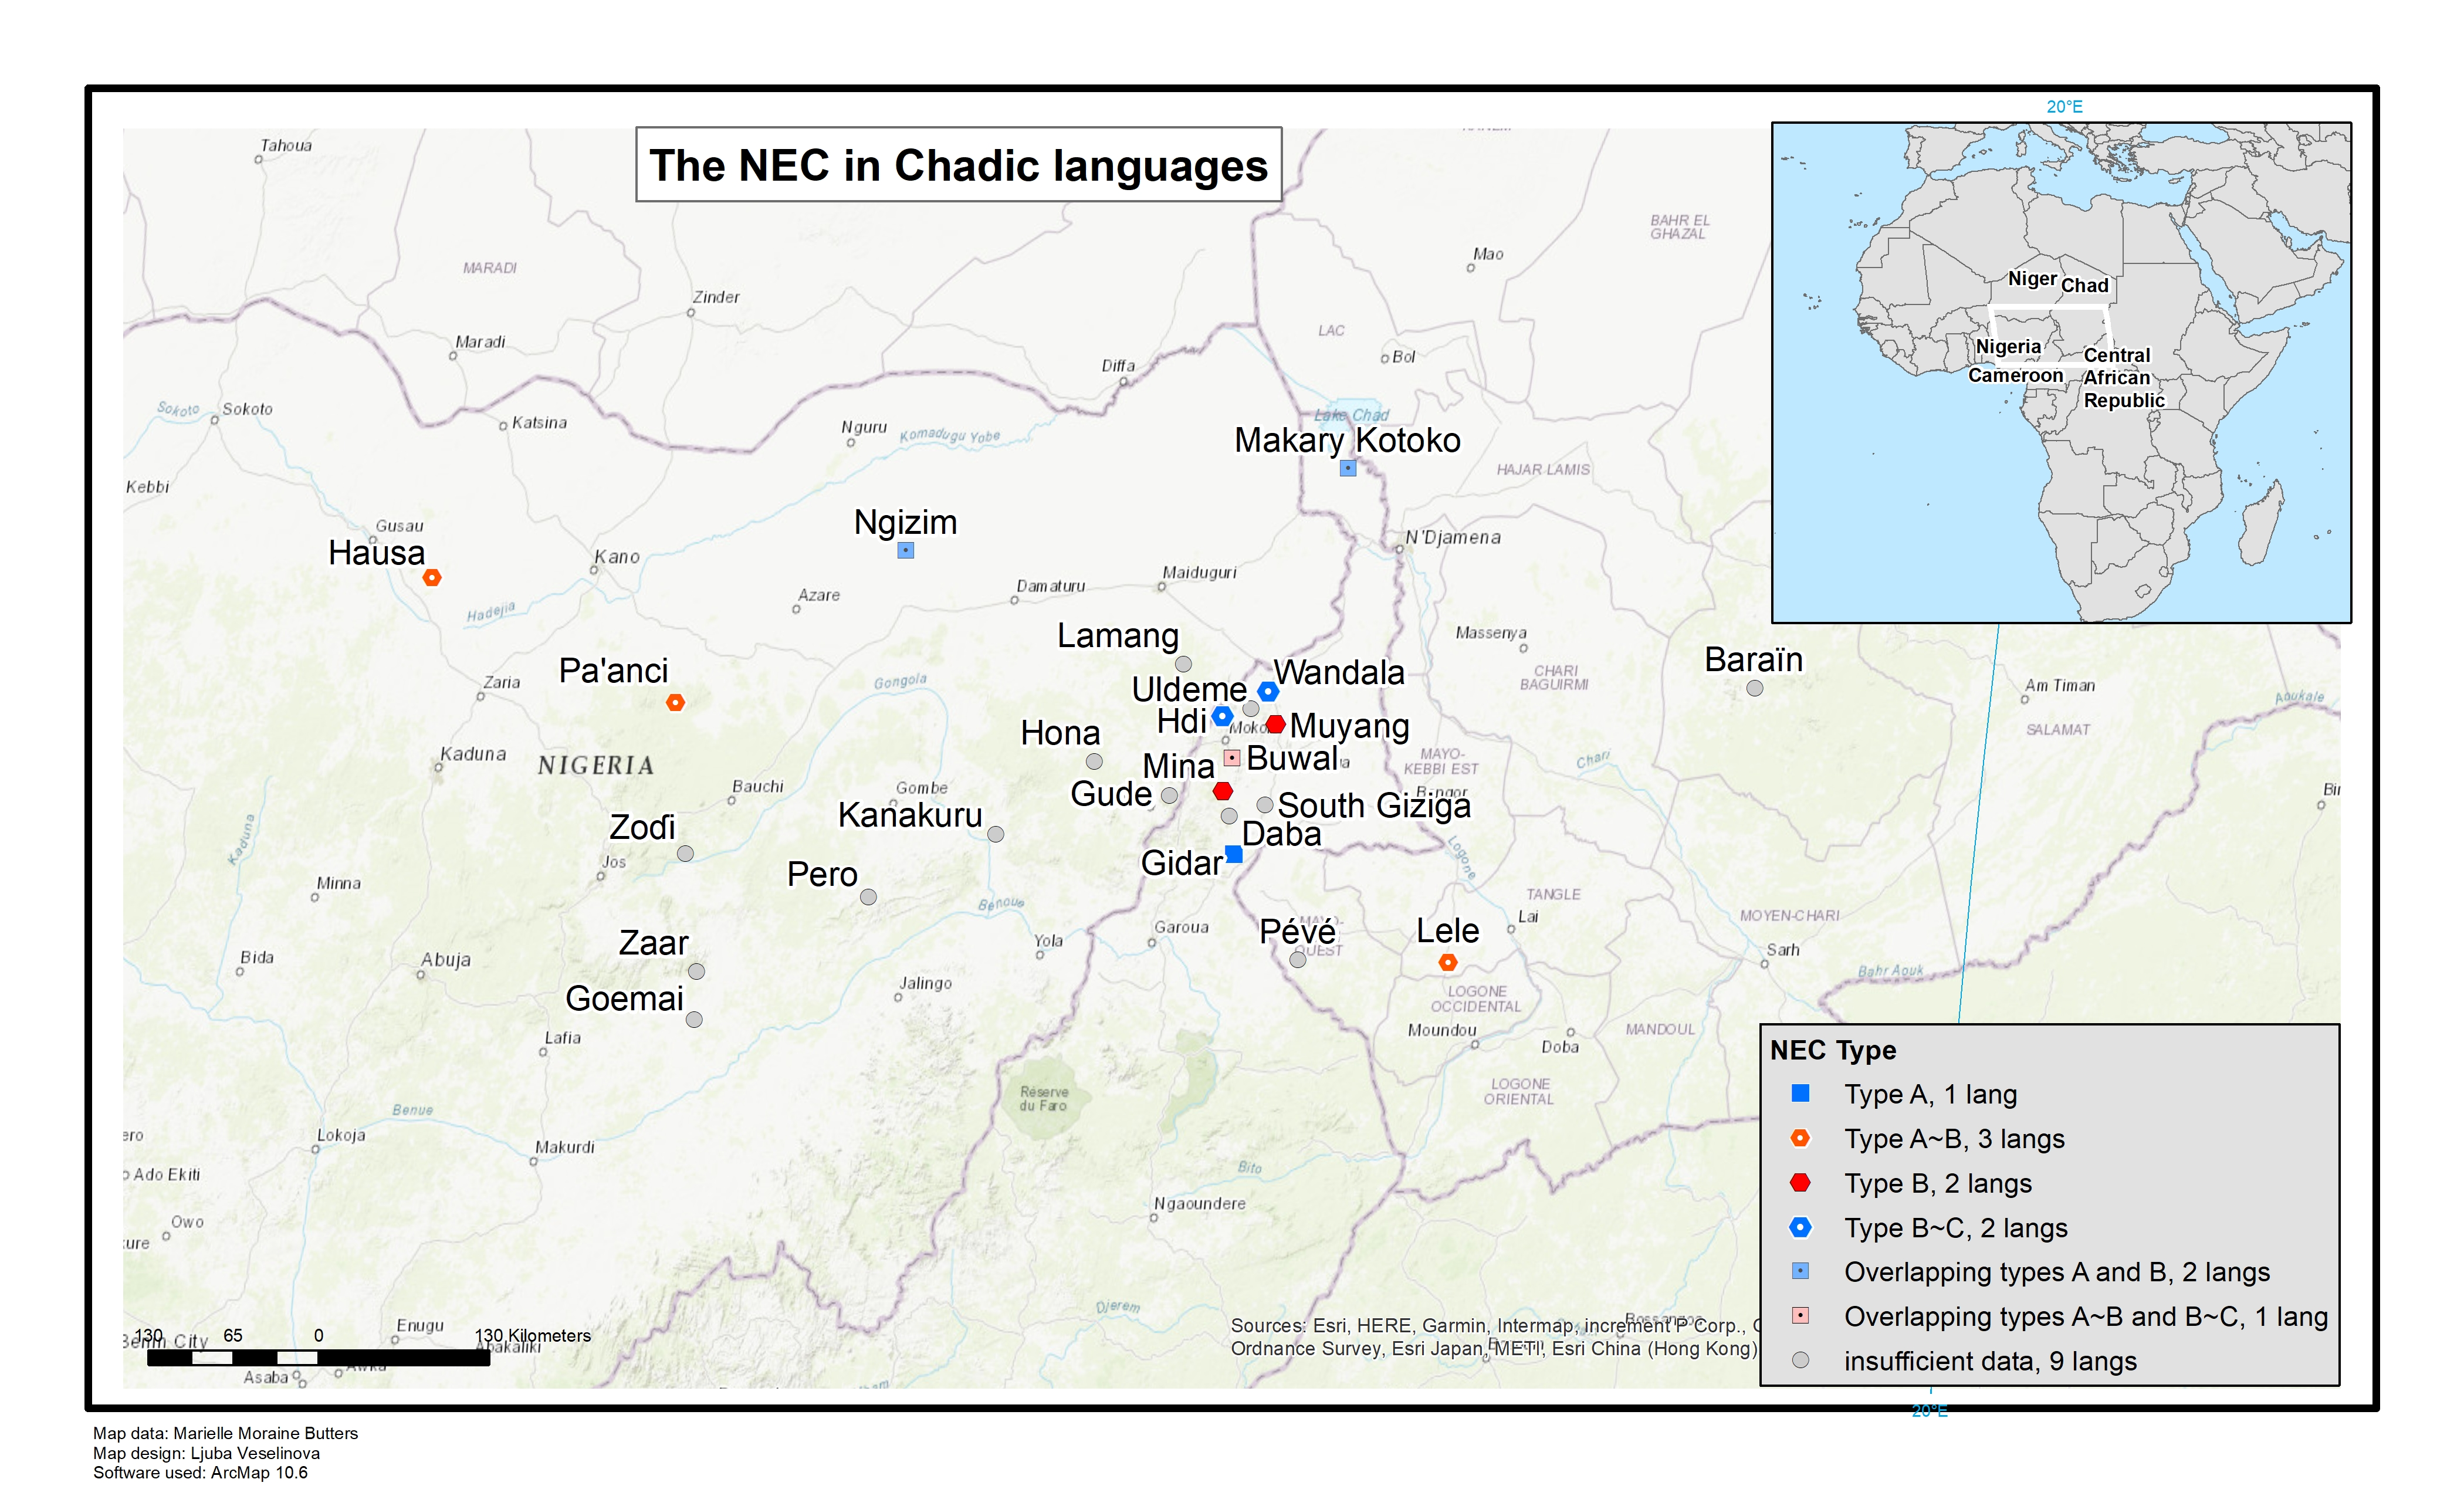
\includegraphics[width=\textwidth]{figures/NEC_in_Chadic.jpg}
    \caption{NEC in Chadic}
    \label{fig:ChadicMap}
\end{sidewaysfigure}

\clearpage

{\sloppy\printbibliography[heading=subbibliography,notkeyword=this]}
\end{document}
